\subsection{Layer Hardware}
Swift Scan app will no longer use a Web Layer to pull and store brewery information records.  The Swift Scan app will pull and store information from an internal text file that'll be created once the user decides to manually add a brewery record or search for a specific brewery product.

\subsection{Layer Operating System}
Swift Scan will execute on Android OS smartphones.

\subsection{Layer Software Dependencies}
Swift Scan will use numerous libraries from the Android API and also several from the Java SDK.  Due to the features that the GUI will provide, the Android API libraries will help accomplish this task and most of the back-end development will be accomplished with libraries from the Java SDK.

\subsection{Subsystem 1}
The Smart scan app will access the database via database connector and will be able to request the required information or make changes.
The databse will send the requested output as required or will allow the user to input new data for the brewery product.
\begin{figure}[h!]
	\centering
 	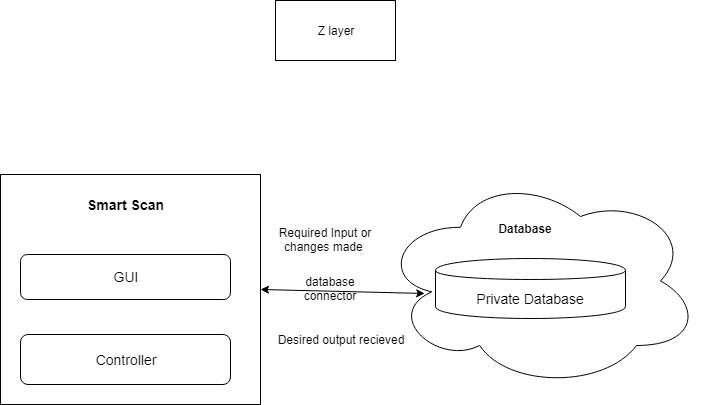
\includegraphics[width=0.60\textwidth]{images/zlayer}
 \caption{Example subsystem description diagram}
\end{figure}

\subsubsection{Subsystem Hardware}
Smart scan will use the devise storage.
\subsubsection{Subsystem Operating System}
A description of any operating systems required by the subsystem.

\subsubsection{Subsystem Software Dependencies}
Any of the class files for Swift Scan will use Android's API along with Java SDK libraries for development of the GUI and back-end development of the functionality of the app, respectively.

\subsubsection{Subsystem Programming Languages}
The main programming language used for the Swift Scan app is Java and using Android's API for the GUI development.

\subsubsection{Subsystem Data Structures}
ASwift Scan will contain two classes to write data to the internal text file and the second class will be used to retrieve the data and display the data to the user.  The second class where the data will be retrieved from the text file will have a method to sort the data as well so it can be displayed to the user.  In addition, the second class will also contain a method for updating any records within the text file, depending on what the user decides to update.

\subsubsection{Subsystem Data Processing}
rder for the brewery data to be recorded in the text file, the user will need to scan first the barcode of the product.  The app will attempt to search for the brewery record in the internal text file and there will be a class that'll perform a linear search through the text file to see if the barcode string exists in the text file.  In case the barcode string does not exist within the text file, the user will be prompted to enter the brewery information into the app and a Java class file will write the data to the text file.  On the other hand, if the barcode string does exist in the text file, a Java class file will use the linear search algorithm to find the record within the text file and return the brewery product information to the user.  All of the data processing for the Swift Scan app will be done with Java class files and the Android API will display the data to the user through the GUI.
